\chapter{Dark Patterns}
The 'Dark Pattern' is a relatively new term. This neologism was firstly used by Harry Brignull in 2010\cite{dark-patterns-arstechnica} when he registered a domain darkpatterns.org. In this domain, Brignull created an online library to share user interface patterns with deceptive characteristics that intentionally confuse and enrol users in unwanted situations. Another purpose of this online library is to shame websites that use dark patterns.

\section{Definition}
Brignull described dark patterns like so: 'Dark Patterns are tricks used in websites and apps that make you do things that you did not mean to, like buying or signing up for something.'\cite{dark-patterns-brignull} Brignull's definition is simplified to understand what dark patterns with ease. However, it does not include all the dark patterns that Brignull describes. For example, there is a dark pattern that purposely focuses users attention on doing one action and distracts their attention from alternatives. Brignull's definition does not imply this example.

A more accurate definition is the one used in the study made by Princeton researchers. They suggest this definition: 'Dark patterns are user interface design choices that benefit an online service by coercing, steering, or deceiving users into making decisions that, if fully informed and capable of selecting alternatives, they might not make.' \cite{dark-patterns-at-scale}
\section{Taxonomy}

Brignull also defined the first types of dark patterns. This list of types is continuously updated when a new type of dark pattern is found. In April 2021, there were twelve different types of dark patterns defined\cite{dark-patterns-brignull-types}.

The researchers from Princeton University have redefined this list considering the results of their study. This list consists of fifteen types of dark patterns and seven broad categories. Their work also differs from the prior work\cite{dark-patterns-brignull,taxonomies-tales,taxonomies-conti} by the new proposed taxonomy. This new taxonomy focuses on the characteristics of dark patterns and cognitive biases that they exploit in users. They used their taxonomy to classify and describe discovered dark patterns.

This thesis uses the same taxonomy defined by Princeton researchers. This taxonomy consists of five dimensions:

\begin{description}
    \item[Asymmetric] \hfill \\ The user interface presents more alternatives to a user. It is an asymmetric characteristic of a dark pattern if the user interface requires less effort to continue with the alternative that might be disadvantageous for users. A typical example is buttons for accepting and rejecting cookies on websites. Usually, the rejecting button is less noticeable. Also, if users want to reject saving cookies, the user interface forces them to read much more text and click many buttons for every single cookie.
    \item[Covert] \hfill \\ The user interface shows evidence of covert characteristics if users may fail to recognise the intended outcome of a specific action. Users have experience with other user interfaces, and they may predict a similar outcome from the interface that shows similar traits as a decoy to influence their decision-making process. For instance, most of the websites offer a subscription to a newsletter in the process of registration. Usually, this subscription to the newsletter is done by ticking a checkbox in the registration form. When users start to read a sentence mentioning the subscription, they automatically expect that not ticking the checkbox means not subscribing to the newsletter.
    \item[Deceptive] \hfill \\ The user interface induces false beliefs in users by presenting them misleading information. For instance, a website may offer a discount for a limited period of time, but in reality, the discount is permanent. Another example is a website that shows how many users are watching the given product and how many products are in stock. This information can take advantage of the deal by steering users into making quick decisions or inducing false beliefs of the product's exclusivity.
    \item[Hides Information] \hfill \\ The user interface intentionally delay presenting necessary information in places or in time, where or when users do not expect them to be presented. For instance, a website may present extra fees for a bought product at the very last step of the checkout.
    \item[Restrictive] \hfill \\ The user interface restricts the set of choices available to users and takes advantage of it. For example, a website may require to sign up only with Facebook to collect additional personal information.
\end{description}

In addition to these dimensions, Princeton researchers define six different effects on users through exploiting different cognitive biases by specific dark patterns:

\begin{itemize}
    \item \textbf{Anchoring Effect}: The tendency of users to over-rely on the first piece of information in the future decision-making process.
    \item \textbf{Bandwagon Effect}: The tendency of users to value more or believe in something simply because others do.
    \item \textbf{Default Effect}: The tendency of users to stick with default options.
    \item \textbf{Framing Effect}: The tendency of users to choose different options with knowledge of the same information, but with a different way of presenting the options.
    \item \textbf{Scarcity Bias}: The tendency of users to value more things that are more sparse.
    \item \textbf{Sunk Cost Fallacy}: The tendency of users to continue an action because they already invested time or other resources in it. Users tend to continue even if that action is capable of putting them in an even worse situation.
\end{itemize}

\section{Categories and types of Dark Patterns}
The types introduced in this section are the same defined in the paper from Princeton university\cite{dark-patterns-at-scale}, but with examples found on the Czech webshops. These types are based on the types firstly published by Harry Brignull\cite{dark-patterns-brignull}.
Princeton researchers discovered 15 types of dark patterns in total, and they divided them into seven broader categories. The summarisation of these types is in table \ref{tab:darkpatterns} at the end of this section.
    \subsection{Sneaking}
    It is an attempt to hide, disguise, or delay information that is relevant to users. Users would likely change their action future action if they knew about this information. There are three types of dark patterns in this category: Sneak into Basket, Hidden Costs, and Hidden Subscription.
        \subsubsection{Sneak into Basket}
        This type of dark pattern adds additional products into the user's basket without their consent. Usually, he is not aware of this fact. The added products are bonuses or additional services — for example, an additional year of warranty or a gift card. The essential for this dark patterns is that it raises the total price, and users might not be aware of this fact. 
        
        This dark pattern exploits the \emph{default effect} of cognitive bias in users that was described earlier in this thesis. The literature says that this dart pattern is not \emph{covert} because users can see the added products in their baskets.

        \begin{figure}[ht]
            \centering
            \frame{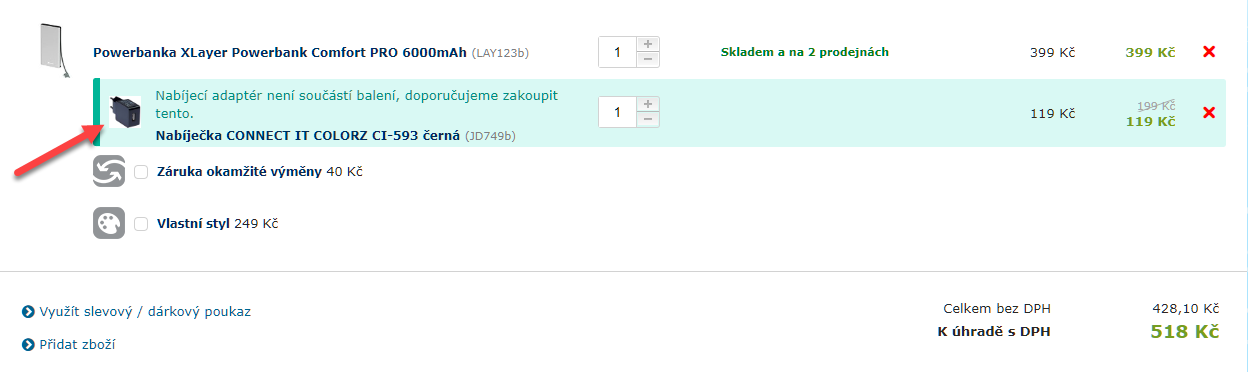
\includegraphics[width=1\linewidth]{media/darkpatterns-examples/sneak-into-basket-alza.png}}
            \caption{An example of Sneak into Basket dark pattern that was used on Alza.cz in 2018, the biggest Czech e-commerce website. The user added a power bank into his basket, and this webshop added a charger into the basket. Alza.cz claimed that users might need these additional buyings because users could not use the bought products without them \cite{alza-sneak-into-basket-idnes}.}
            \label{fig:alza-sneak-into-basket}
        \end{figure}

        \subsubsection{Hidden Cost}
        This pattern is an attempt to add additional charges, typically at the end of the purchase process. Typical examples of this type of dark pattern are additional service fees or handling costs. 
        
        This type of dark pattern is also not \emph{covert}, but it may be considered partially \emph{deceptive} because the information is delayed from users. Also, this dark pattern can be classified into \emph{hides information} dimension, as it attempts to hide information from users.
        \begin{figure}[ht]
            \centering
            \frame{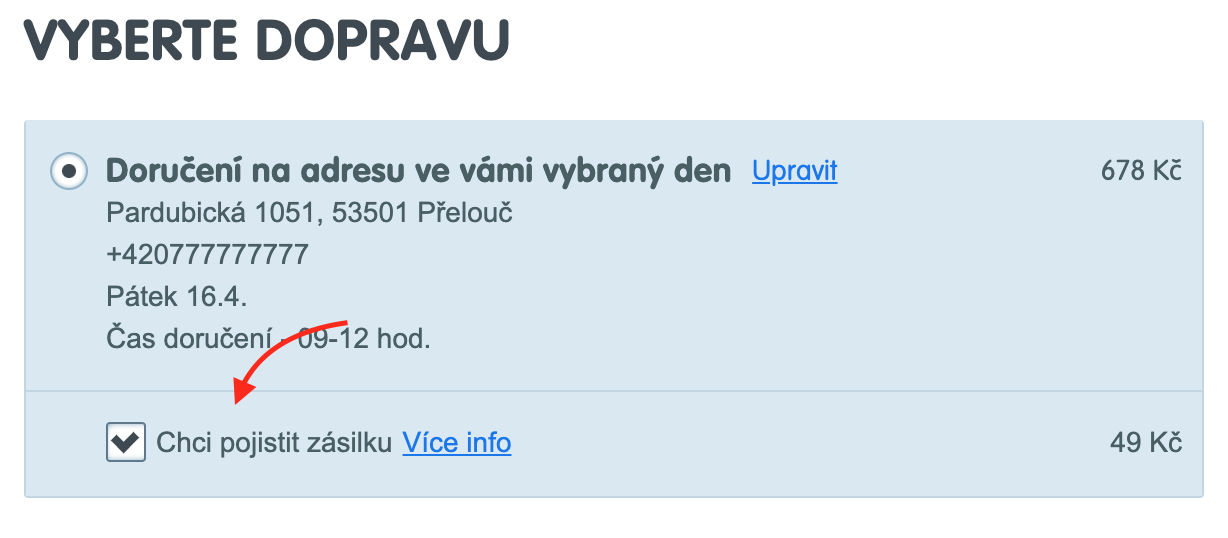
\includegraphics[width=1\linewidth]{media/darkpatterns-examples/hidden-cost-mall.png}}
            \caption{An example of Hidden Cost dark pattern that appears at the very last step of the purchase flow on Mall.cz. This webshop adds a payment for insurance, which users may not notice. "Chci pojistit zásilku" can be translated as "I want to insure the shipment".}
            \label{fig:hidden-cost-mall}
        \end{figure}

        \subsubsection{Hidden Subscription}
        This pattern signs up users into a subscription with a recurring fee. Users may not be aware of this subscription because the subscription is presented as a one-time payment or a free trial. This type of dark pattern usually appears together with another dark pattern named 'Hard to Cancel'. 
        
        \begin{figure}[ht]
            \centering
            \frame{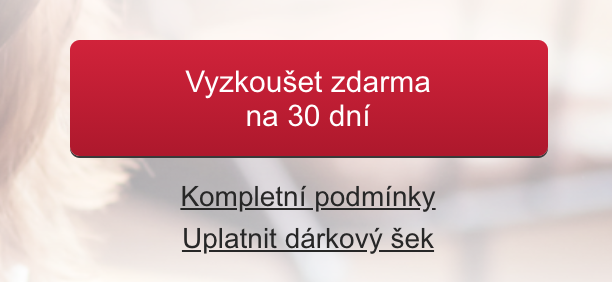
\includegraphics[width=0.5\linewidth]{media/darkpatterns-examples/hidden-subscription-alza.png}}
            \caption{An example of Hidden Subscription that was used by Alza.cz in 2016\cite{hidden-subscription-alza-2016}. Alza promoted 30 days free of its VIP membership. If users did not cancel their membership within those 30 days, Alza assumed that users were interested in continuing their membership and paying the fee.}
            \label{fig:hidden-subscription-alza}
        \end{figure}

        This dark pattern is classified to be partially \emph{deceptive} because it may confuse and mislead users. Also, it can be said that this dark pattern \emph{hides information} from users.
    \subsection{Urgency}
    Dark patterns from this category speed-up users decision-making process by exploiting scarcity bias in users. For example, this can be done by showing more beneficial or time-limited discounts to users. As a result, users value products more than they would normally do. These dark patterns usually keep signalling that the special offer may be lost to users if they do not react promptly. This dark pattern is usually combined together with 'Social Proof' and 'Scarcity' types of dark patterns defined below.
        \subsubsection{Countdown Timers}
        This dark pattern is usually in the form of an indicator of a deadline, counting down to the end of the deadline. 
        
        This dark pattern is classified as partially \emph{covert} because it evokes untrue feelings of immediacy in users and is sometimes classified as \emph{deceptive} because the indicator sometimes shows false information. For example, the timer can reset every time it reaches the deadline.

        \begin{figure}[ht]
            \RawFloats
            \begin{minipage}[t]{0.52\linewidth}
                \strut\vspace*{-\baselineskip}\newline
                \frame{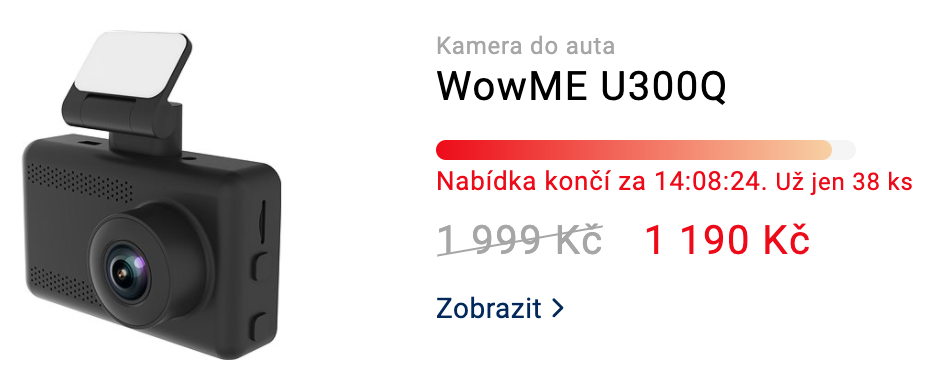
\includegraphics[width=1\linewidth,valign=t]{media/darkpatterns-examples/countdown-timers-alza1.png}}
                \caption{An instance of 'Countdown Timers' dark pattern on Alza.cz's homepage. The caption "Nabídka končí za 14:08:24" can be translated as "The offer ends in 14:08:24". changes this offer for a different product every day.}
                \label{fig:countdown-timers-alza1}
            \end{minipage}
            \hfill
            \begin{minipage}[t]{0.44\linewidth}
                \strut\vspace*{-\baselineskip}\newline
                \frame{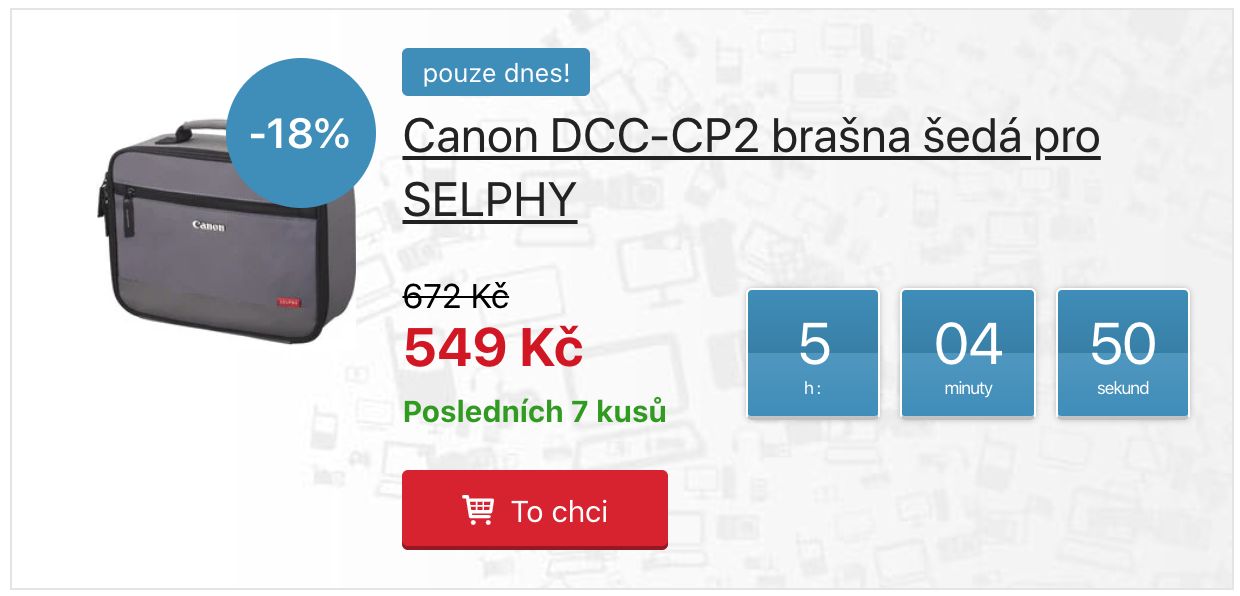
\includegraphics[width=1\linewidth,valign=t]{media/darkpatterns-examples/countdown-timers-czc.png}}
                \caption{Another instance of 'Countdown Timers' dark pattern, but this was found on CZC.cz homepage.}
                \label{fig:countdown-timers-czc}
            \end{minipage}
        \end{figure}

        \subsubsection{Limited-time Messages}
        The 'Limited-time message' dark pattern differs from 'Countdown Timer' by static urgency message and not showing the exact time of the deadline. 
        
        With the taxonomy defined before, this dark pattern is classified as \emph{covert} because of the same reason as 'Countdown Timer' dark pattern and \emph{information hiding} because it does not show the deadline in its offers.

        \begin{figure}[ht]
            \centering
            \frame{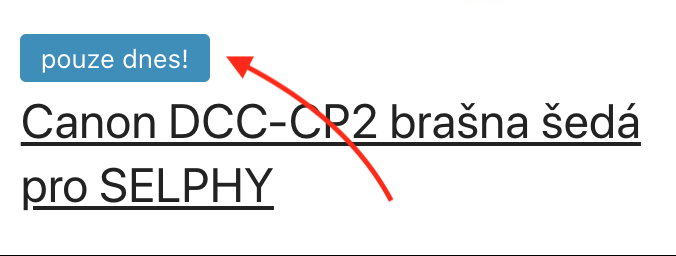
\includegraphics[width=0.60\linewidth]{media/darkpatterns-examples/limited-time-message-czc.png}}
            \caption{An instance of 'Limited-time message' dark pattern found on a product page of CZC.cz webshop. The red arrow is pointing at the caption "pouze dnes!", which can be translated as "only today!".}
            \label{fig:limited-time-message-czc}
        \end{figure}

    \subsection{Misdirection}
    This category of dark patterns uses visuals and language to distract users' attention on other possible presented choices. Also, some types from this category use users' emotions to invoke bad feelings of being guilty or ashamed for not making a specific choice. Users trust or feel that the other choices are unavailable or less beneficial for them. Essential for this dark pattern is that other choices are not hidden. Users are aware of the other choices, but this category of dark patterns steers users away from the other choices. Princeton researchers discovered four types of dark patterns from this category: 'Confirmshaming', 'Visual Interference', 'Trick Questions', and 'Pressured Selling'.
        \subsubsection{Confirmshaming}
        The 'Confirmshaming' dark pattern uses language and emotions to focus the attention of users on one choice in order to distract attention on other choices. Researchers point out that this dark pattern usually appeared in popup dialogues that asked for an email address in exchange for a discount. Some instances of this dark pattern evoke emotions of shame in users if they select an option that webshop do not want them to select. Typical examples of such option is 'No, I want to pay full price' or 'No thanks, I hate saving money'. This dark pattern exploits the framing effect of cognitive bias in users by presenting choices differently to users.
        
        Thus, this dark pattern is classified as \emph{asymmetric}. However, it is not \emph{covert} since all the possible choices are presented to users.

        \subsubsection{Visual Interference}
        The 'Visual Interference' dark pattern uses different styles and visuals to draw users' attention to certain choices - the choices that the website wants users to choose. A typical example of this dark pattern is two buttons in different styles for opting-in and opting-out for the website's newsletter subscription. One of the buttons - the one that the website wants users to click on - looks more promising, more attractive to users' eyes than the other one. The different styles steer users attraction to the opting-in choice. 
        
        By provided taxonomy, this type of dark pattern is partially classified as \emph{asymmetric} because it sometimes unequally present choices to users. Users may not realise that the effect of the dark pattern influenced them. Because of this fact, this dark pattern is also classified as \emph{covert}. Some instances can be also classified as \emph{deceptive}, and Princeton researchers give an example of an option "lucky draw" among others that are deterministic and not random.
        
        \begin{figure}[ht]
            \centering
            \frame{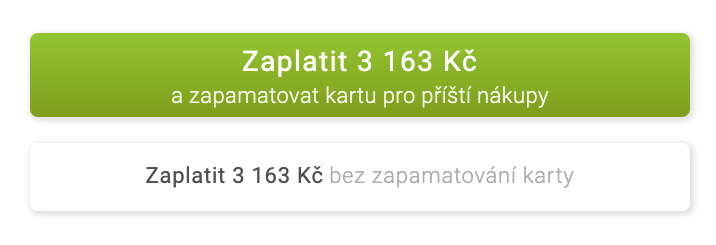
\includegraphics[width=0.7\linewidth]{media/darkpatterns-examples/visual-interference-alza.png}}
            \caption{An instance of 'Visual Interference' dark pattern on Alza.cz. This instance appears in the last step of the buying process, where users fill in their payment information. Alza.cz steers users' attention to the option with the green background "Zaplatit 1 249 Kč a zapamatovat kartu pro příští nákupy" (English: "Pay 1 249 CZK and save the card information for the future payments") and hides the other option, by which users would not approve to save the card information.}
            \label{fig:visual-interference-alza}
        \end{figure}

        \subsubsection{Trick Questions}
        The 'Trick Question' dark pattern uses confusing language to confuse users and their ability to make decisions. A typical trick in the English language for this dark pattern is double negatives. For example, websites, using this type of dark pattern, invert the meaning of a check subscription checkbox, usually seen in registration forms, followed with confusing language 'Uncheck this box if you prefer not to receive email updates'. Users need to pay more attention to properly understand which state of the checkbox means the subscription for the newsletter and which not. This type of dark pattern exploits the default effect in users, who erroneously believe that to them presented user interface follows traditional patterns. Also, this dark pattern exploits the framing effect by presenting the same information in a different, more confusing way to influence users in choosing different choices.
        
        Therefore, Princeton researchers classify this type of dark pattern as \emph{asymmetric} because opting out takes more effort than opting in. Also, researchers classify this dark pattern as \emph{covert} because users may falsely understand the effect of their choice.

        \begin{figure}[ht]
            \centering
            \frame{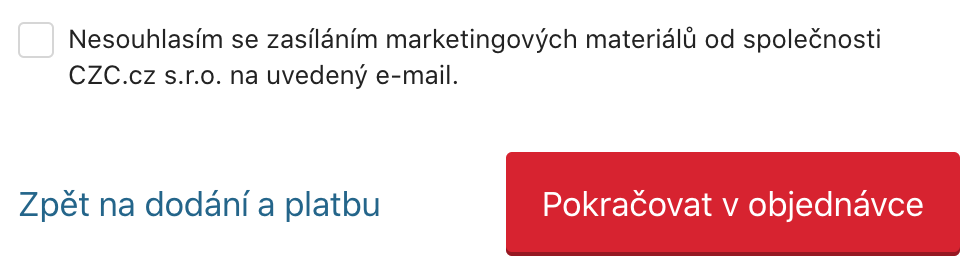
\includegraphics[width=0.8\linewidth]{media/darkpatterns-examples/trick-questions-czc.png}}
            \caption{An instance of 'Trick Questions' dark pattern on CZC.cz, where "Nesouhlasím se zasíláním marketingových materiálů ..." can be translated as "I do not agree with ..." While this sentence is not a question, it is certainly confusing because users must indicate their opposition to the newsletter subscription.}
            \label{fig:trick-questions-czc}
        \end{figure}

        \subsubsection{Pressured Selling}
        Princeton researchers define the 'Pressured Selling' dark pattern as pre-selecting more expensive variations of the same product as default. Additionally, pressuring users into choosing the more expensive variations or buying related products is also considered as a tactic of this dark pattern. More cognitive biases are triggered and exploited by this dark pattern, such as the default effect, the anchoring effect (users may tend to overlook the other choices) and the scarcity bias (more expensive variations may seem to be more exclusive).  
        
        This dark pattern is for some instances classified as \emph{asymmetric} (i.e., steering users and their acceptance towards more expensive options), and partially \emph{covert} (users may fail to realise that the firstly shown price of the less expensive variation of the product is not the same price, as the more expensive default variation).

        \begin{figure}[ht]
            \RawFloats
            \centering
            \begin{minipage}[ht]{0.55\linewidth}
                \strut\vspace*{-\baselineskip}\newline
                \centering
                \frame{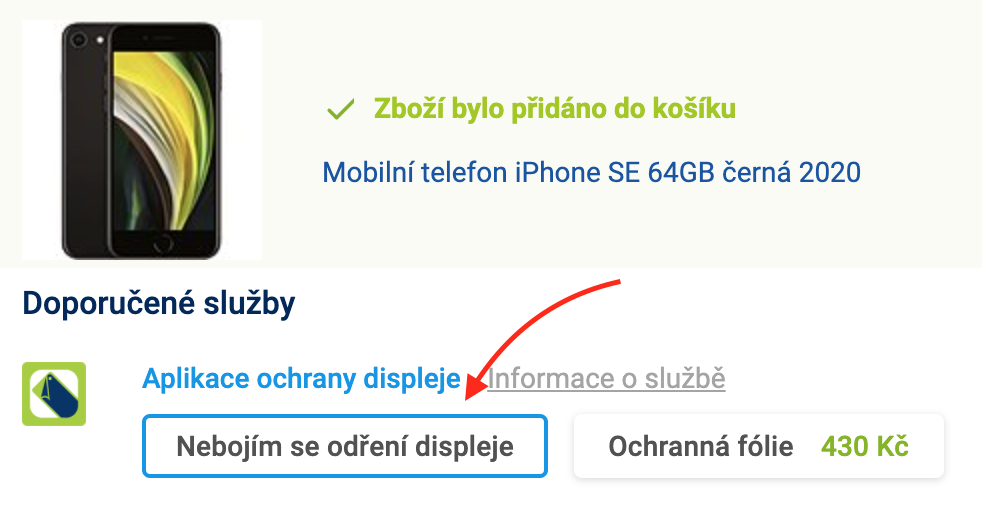
\includegraphics[width=1\linewidth]{media/darkpatterns-examples/pressured-selling-alza1.png}}
                \caption{An instance of 'Pressured selling' dark pattern found on Alza.cz again. Webshop offers additional services (a protective glass in this instance) for products in the basket. Webshop preselected an option "Nebojím se odření displeje" (English: "I am not worried about the scratches on the display"), which is intended to evoke worries and scare emotions in users.}
                \label{fig:pressured-selling-alza1}
            \end{minipage}
            \hfill
            \begin{minipage}[ht]{0.40\linewidth}
                \strut\vspace*{-\baselineskip}\newline
                \centering
                \frame{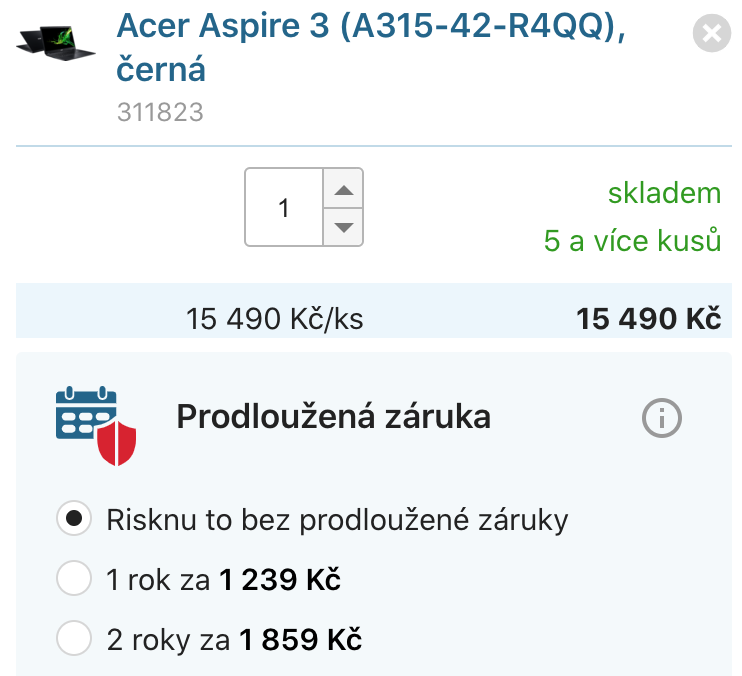
\includegraphics[width=1\linewidth]{media/darkpatterns-examples/pressured-selling-czc.png}}
                \caption{Another similar instance of 'Pressured selling' dark pattern. This instance was found on CZC.cz. "Risknu to bez prodloužené záruky" can be translated as "I will take my chances without the extended warranty."}
                \label{fig:pressured-selling-czc}
            \end{minipage}
            \begin{minipage}[ht]{1\linewidth}
                \vspace{0.3cm}
                \centering
                \frame{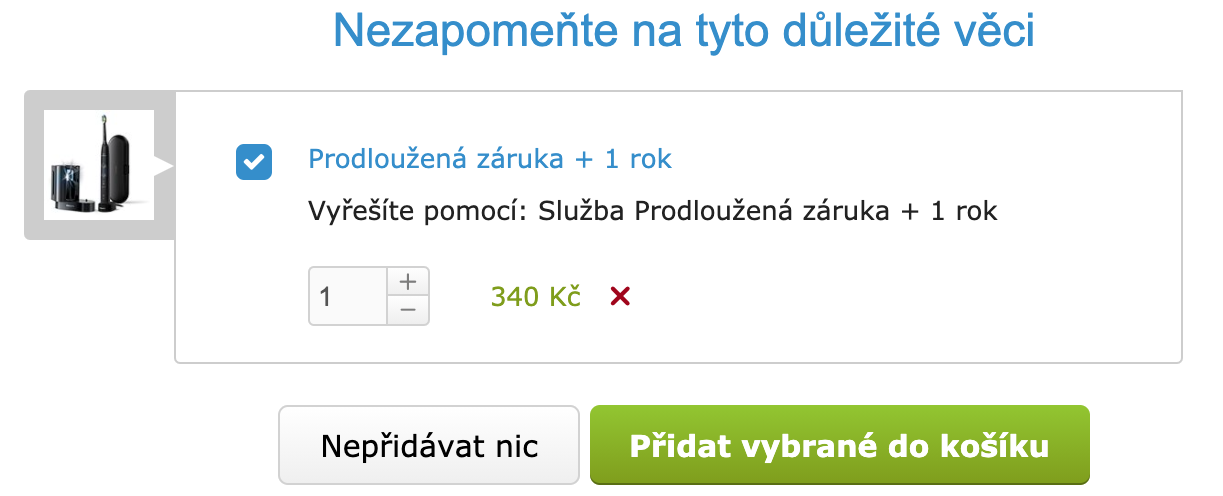
\includegraphics[width=0.7\linewidth]{media/darkpatterns-examples/pressured-selling-alza2.png}}
                \caption{The third instance of 'Pressured selling' dark pattern. This instance is a modal window, that occasionally pops up right after the confirmation of the content of the basket. The headline says: "Do not forget these important additional products." The webshop preselects these additional products. In this example, there is 'Visual Interference' dark pattern as well. The styling of the acceptance button (the green button) tempts users to click on particular button.}
                \label{fig:pressured-selling-alza2}
            \end{minipage}
        \end{figure}

    \subsection{Social Proof}
    The 'Social Proof' category of dark patterns is based on a social proof principle. Those hesitating individuals, who do not know what to do in a given situation, tend to observe others and mimic their moves, actions, and behaviour \cite{influence-cialdini, evilbydesign}. This category of dark patterns misuses this behaviour of individuals, and it exploits the bandwagon effect of cognitive bias to its advantage. Princeton researchers define two types from this category: Activity Notifications and Testimonials of Uncertain Origin.

        \subsubsection{Activity Notifications}
        The 'Activity Notifications' dark pattern is information on product pages that indicate other users' activity. The message can have different forms. It can be a number of other users watching the same product or a number of sold products to other users. Messages displaying recent purchases of other users (e.g., 'User X just bought a product Y') also counts as 'Activity Notifications' dark pattern. Princeton researchers point out that some websites claim activity that is deceptive and not true. These websites use a misleading random number instead of factual information. This number also changes after some time, making it even more challenging to recognise as deceptive. 

        \begin{figure}[ht]
            \RawFloats
            \centering
            \begin{minipage}[ht]{0.55\linewidth}
                \strut\vspace*{-\baselineskip}\newline
                \centering
                \frame{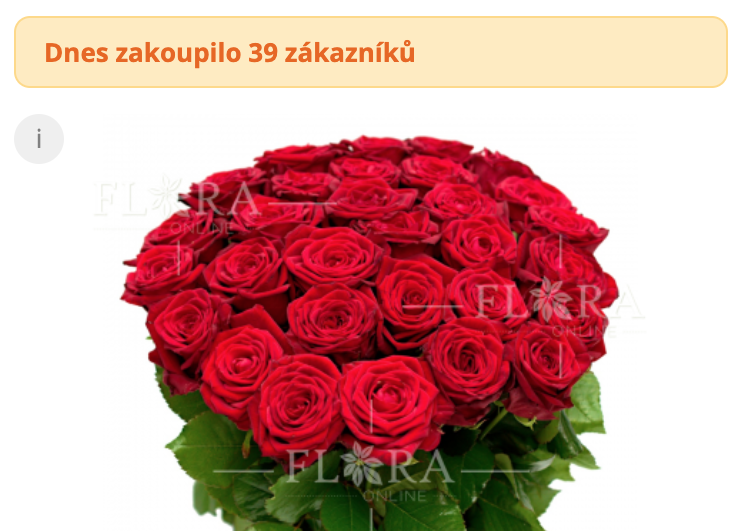
\includegraphics[width=1\linewidth]{media/darkpatterns-examples/activity-notifications-flora-online.png}}
                \caption{An instance of 'Activity Notifications' dark pattern on flora-online.cz, where "Dnes zakoupilo 31 zákazníků" can be translated as "31 customers bought this product today".}
                \label{fig:activity-notifications-flora-online}
            \end{minipage}
            \hfill
            \begin{minipage}[ht]{0.40\linewidth}
                \strut\vspace*{-\baselineskip}\newline
                \centering
                \frame{
\includegraphics[width=1\linewidth]{media/darkpatterns-examples/activity-notifications-kytice-expres.png}}
                \caption{Another instance of 'Activity Notification' dark pattern. This instance was found on kytice-expres.cz. It shows the recently bought flowers by other users."}
                \label{fig:pressured-selling-czc}
            \end{minipage}
        \end{figure}

        Some instances of this dark pattern can be classified as \emph{covert} because users fail to understand that this dark pattern influences their decision-making process in a way that they tend to buy a product, which is sold more often or is viewed more by other users. Also, some instances are classified as \emph{deceptive} because they present made up untruthful information and users are not aware of this fact.

        \subsubsection{Testimonials of Uncertain Origin}
        This type of dark pattern refers to the use of customer testimonials whose origin is unclear and not sourced enough. The result of such testimonials is that users' decision-making process is influenced by untrue information, and they erroneously believe in the quality of products. In addition, a new directive will apply to all EU member states in 2022. This directive demands all e-shops to state how they ensure the authenticity of references\cite{penize-testimonials}.
        
        \begin{figure}[ht]
            \centering
            \frame{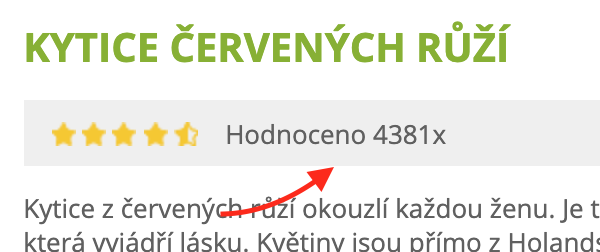
\includegraphics[width=0.6\linewidth]{media/darkpatterns-examples/testimonials-kytice-expres.png}}
            \caption{An example of Testimonials of Uncertain Origins dark pattern found on kytice-expres.cz. The webshop claims 4381 rankings of a product (czech: "Hodnoceno 4381x") with an average score of four and a half stars out of five. There was no additional information on how the webshop obtained these references.}
            \label{fig:testimonials-kytice-expres}
        \end{figure}

        Using taxonomy defined by Princeton researchers, this dark pattern is classified as sometimes \emph{deceptive}, and it depends on the truthfulness of the testimonials, which can be determined by scanning the website and looking for a submission form for sending testimonials.


    \subsection{Scarcity}
    The 'Scarcity' category contains such types of dark pattern that implement messages indicating limited availability or high demand for a product. Thus, the value of the product increases because of its exclusivity. This dark pattern forces users to make quicker decisions. Users may feel intimidated by losing the chance to buy this very desirable product because it could be sold out soon. Princeton researchers define two types of dark patterns: 'Low-stock Message' and 'High-demand Message'.
        \subsubsection{Low-stock Message}
        The 'Low-stock Message' dark pattern informs users about the limited availability of a product; thus, users want to prevent losing the chance to buy the product by making quicker decisions than they normally do. Some instances of this dark pattern show exact quantities left on the stock. Others only show a message that stock is almost empty. This dark pattern exploits scarcity bias in users - making products more valuable only because it is low on stocks. Some websites use untruthful data to keep arousing the feelings of need in users all the time.

        \begin{figure}[ht]
            \centering
            \frame{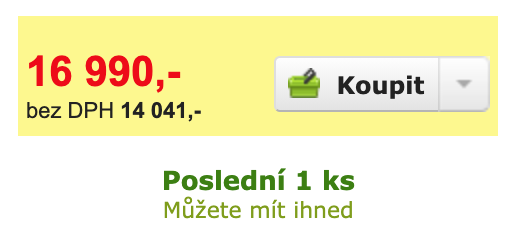
\includegraphics[width=0.4\linewidth]{media/darkpatterns-examples/low-stock-messages-alza1.png}}
            \caption{An instance of 'Low-stock Message' dark pattern on Alza.cz. The green text "Poslední 1 kus" can be translated as "The last 1 product left in stock".}
            \label{fig:low-stock-messages-alza1}
        \end{figure}

        Princeton researchers classify the 'Low-stock Message' dark pattern as partially \emph{covert} because users fail to realise that these messages influenced their decision-making process. Some instances of this dark pattern are classified as \emph{deceptive} for displaying false information to users about being low on stock, but it is not. Some other instances are classified as \emph{information hiding} for hiding the exact quantities of the product on stock.

        \subsubsection{High-demand Message}
        The 'High-demand Message' dark pattern informs users that a product is in high demand and can be sold out soon.

        Similarly to 'Low-stock Message' dark pattern, 'High-demand Message' is also classified as partially \emph{covert}.

        \begin{figure}[ht]
            \centering
            \frame{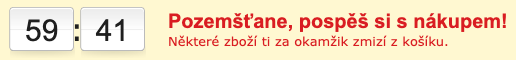
\includegraphics[width=0.7\linewidth]{media/darkpatterns-examples/high-demand-message-alza.png}}
            \caption{An instance of 'High-demand Message', that can be found in the basket of Alza.cz webshop. It can be translated as "Dear stranger, hurry up! Some of the goods from your basket may disappear soon!"}
            \label{fig:high-demand-message-alza}
        \end{figure}

    \subsection{Obstruction}
    This 'Obstruction' category contains only one type of dark pattern, which is 'Hard to Cancel'. This type of dark pattern refers to make specific actions harder to complete than other actions. For instance, signing up for a subscription to an annually paid service is often much more straightforward than cancelling the subscription \cite{unbounce-subscription}. Also, Princeton researchers mention examples when cancellation of a subscription is available only by calling customer service\cite{dark-patterns-at-scale}.

    This dark pattern is sometimes classified as \emph{restrictive} with the defined taxonomy because it restricts the available choices to cancel the previous subscriptions. The 'Hard to Cancel' dark pattern becomes \emph{information hiding} when the website does not inform users how to cancel the subscription or about the fact that cancellation is not as easy as signing up.

    \begin{figure}[ht]
        \centering
        \frame{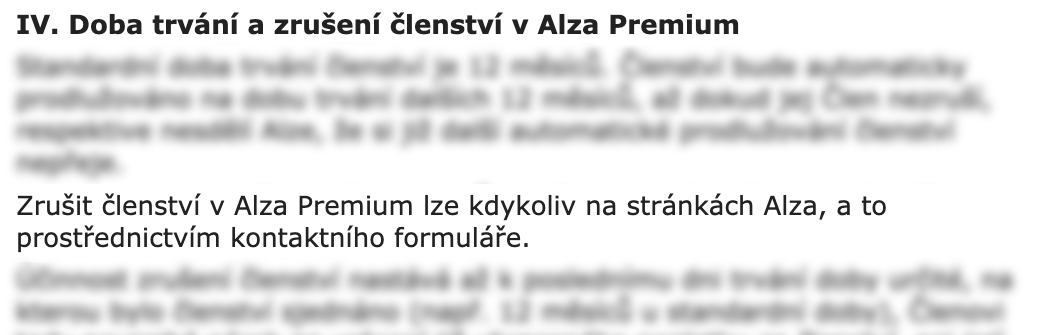
\includegraphics[width=0.7\linewidth]{media/darkpatterns-examples/hard-to-cancel-alza.png}}
        \caption{Example of Hard to Cancel dark pattern in Alza Premium terms of service. If users want to cancel the auto-renewal service, they need to contact customer care via the contact form. The translation of the bottom paragraph from the terms of service is: "Alza Premium membership can be cancelled at any time on the Alza website via the contact form."}
        \label{fig:hard-to-cancel-alza}
    \end{figure}

    \subsection{Forced Action}
    The 'Forced Action' dark pattern category forces users to take additional action, even though they might not normally take it to finish their task. The 'Forced Enrollment' is the only type of dark pattern discovered and defined by Princeton researchers in this category. This type of dark pattern forces users (that want to use the service) into enrolling for a marketing newsletter or into creating accounts, which gives the website more information than is needed to use the service. Princeton researchers describe an example when users have to simultaneously sign up for a marketing newsletter alongside their consent to terms of service.

    Princeton researchers define this type of dark pattern as \emph{assymetric}, because of the requirement of the additional actions to complete users' tasks, which creates asymmetrically balanced choices, and \emph{restrictive}, because it forces users into creating accounts and signing up for marketing newsletters.

    \begin{figure}[ht]
        \centering
        \frame{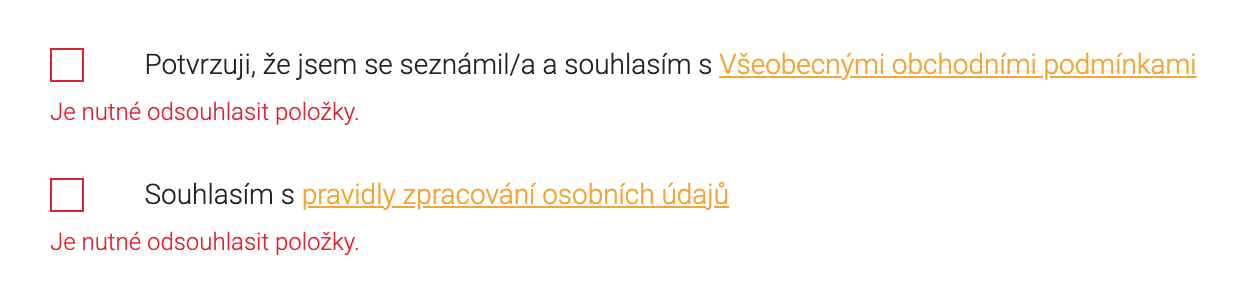
\includegraphics[width=0.8\linewidth]{media/darkpatterns-examples/forced-enrollment-bestdrive.png}}
        \caption{An example of Forced Enrollment that can be found on registration page of bestdrive.cz. By checking the first checkbox, users confirm their acceptance of the general terms of use. By checking the second checkbox, they agree to the processing of personal data, which also leads to the subscription.}
        \label{fig:forced-enrollment-datart}
    \end{figure}

\begin{table}
    \centering
    \caption{Summarisation of categories and types of dark patterns with their description, definition and cognitive biases they exploit \cite{dark-patterns-at-scale}.}\label{tab:darkpatterns}
    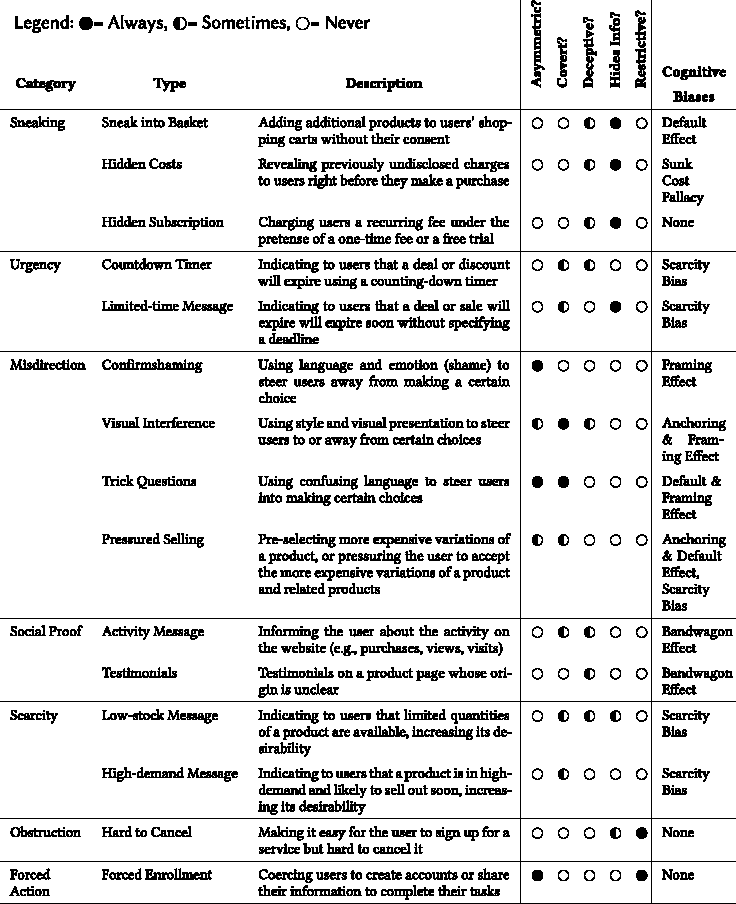
\includegraphics[width=1\textwidth]{media/dp-table.pdf}
\end{table}